\chapter{Zeemann-Effekt}
Für den Übergang von Cadmium $5^1D_2 \rightarrow 5^1P_1$ wird der normale \texttt{Zeemann}-Effekt untersucht. Dafür folgt zunächst ein theoretischer Einschub.
% -----
\section{Theoretischer Hintergrund}

Der \texttt{Zeemann}-Effekt beschreibt die Aufspaltung von Spektrallinien, und somit Aufhebung der Entartung der Energieniveaus gleicher Gesamtdrehimpulse $J$, in einem externen Magnetfeld. 
Diese Aufspaltung ist auf die Wechselwirkung des magnetischen Moments der Atome mit dem äußeren Magnetfeld zurückzuführen.
Unterschieden wird zwischen dem \textit{normalen} ($S=0$) und dem \textit{anormalen} ($S\neq 0$) \texttt{Zeemann}-Effekt.\\
Da beide Niveaus des Cd einen Gesamtspin von $S=0$ besitzen, ist nur der normale \texttt{Zeemann}-Effekt relevant.
Der Hamiltonian des Elektrons im Atom und im Magnetfeld folgt mit:
%--
\begin{equation}
    \widehat{H}= 
    \underbrace{-\frac{\hbar}{2m}\vec{\nabla}^2 
    -\frac{e^2}{4\pi\varepsilon_0 r}}_{\raisebox{1.5ex}{\scriptsize $H_\mathrm{0}$}} 
    \underbrace{+\beta\frac{\hat{\vec{L}}\cdot\hat{\vec{S}}}{\hbar^2}}_{\raisebox{1.5ex}{\scriptsize $H_{\mathrm{Spin-Bahn}}$}}
    \underbrace{+\mu_B\frac{\hat{\vec{L}}+2\hat{\vec{S}}}{\hbar}\vec{B}}_{\raisebox{1.5ex}{\scriptsize $H_{\mathrm{Zeemann}}$}}
\end{equation}
%--
mit dem \textit{Spin-Bahn}-Kopplungsterm $H_{\mathrm{Spin-Bahn}}$ aus der Feinstruktur und dem \textit{Zeemann}-Kopplungsterm $H_{\mathrm{Zeemann}}$ aus der 
Wechselwirkung mit dem äußeren Magnetfeld mit Richtung $\vec{B}=B\vec{e}_z$.\\
Da jedoch $S=0$ fallen einige Terme weg. Die guten Quantenzahlen, also die, die sich nicht ändern, sind $L$, $S$, $J$ und $M_J$ (wobei $J=L+S=L$) und die 
Energiekorrektur zum Hamiltonian ist:
%--
\begin{equation}
    \Delta E = \mu_B g_J M_J B
\end{equation}
%--
mit dem Bohrschen Magneton $\mu_B = \frac{e\hbar}{2m}$ und dem Landé-Faktor $g_J$:
%--
\begin{equation}
    g_J = 1 + \frac{J(J+1) + S(S+1) - L(L+1)}{2J(J+1)}
\end{equation}
%--
Die Aufspaltung der Energieniveaus und möglichen Übergänge für die verschiedenen $M_J$ anhand der Auswahlregeln
%--
\begin{align*}
    \Delta J &= 0, \pm 1\\
    \Delta M_J &= 0, \pm 1
\end{align*}
%--
sind in \cref{fig:cd_niveaus} dargestellt.
%--
\vspace{0.3cm}\\
Die Polarisation der Strahlung hängt von der Änderung der magnetischen Quantenzahl $M_J$ im Übergang ab (siehe \cref{fig:polarisation}):
%--
\begin{itemize}
    \item \textbf{$\pi$-Übergänge:} $\Delta M_J = 0$ — linear polarisiert parallel zur Magnetfeldrichtung
    \item \textbf{$\sigma^+$-Übergänge:} $\Delta M_J = +1$ — rechtszirkular polarisiert (bei longitudinaler Beobachtung)
    \item \textbf{$\sigma^-$-Übergänge:} $\Delta M_J = -1$ — linkszirkular polarisiert (bei longitudinaler Beobachtung)
\end{itemize}
%--
Je nach Beobachtungsrichtung relativ zum Magnetfeld lassen sich unterschiedliche Polarisationen der emittierten Strahlung beobachten:
%--
\begin{itemize}
    \item \textbf{Longitudinale Konfiguration:} Magnetfeld $B$ ist parallel zur Beobachtungsrichtung. Es treten ausschließlich zirkular polarisierte Anteile auf ($\sigma^+$ und $\sigma^-$).
    \item \textbf{Transversale Konfiguration:} Magnetfeld $B$ ist senkrecht zur Beobachtungsrichtung. Es treten linear polarisierte Komponenten auf ($\pi$- und $\sigma$-Komponenten).
\end{itemize}
%--
\begin{figure}[h]
    \centering
    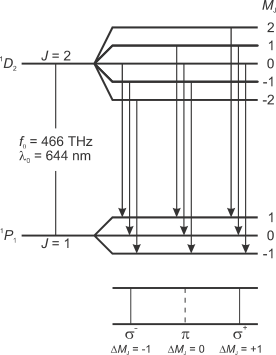
\includegraphics[]{Niveauaufspaltung_Cd.png}
    \caption[Niveauaufspaltung des$5^1D_2 \rightarrow 5^1P_1$-Übergangs bei Cd]{Niveauaufspaltung des $5^1D_2 \rightarrow 5^1P_1$-Übergangs beim normalen \texttt{Zeemann}-Effekt an Cadmium \autocite{LD}}
    \label{fig:cd_niveaus}
\end{figure}
%--
\begin{figure}[h!]
    \centering
    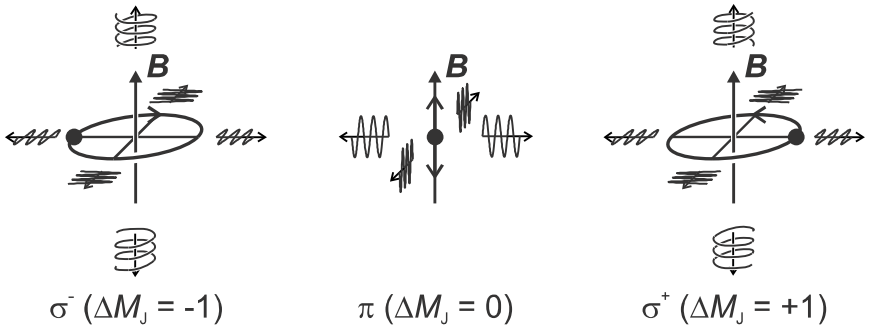
\includegraphics[width=.8\linewidth]{Dipolstrahlung_Verteilung.PNG}
    \caption[Winkelverteilung der elektischen Dipolstrahlung]{Winkelverteilung der elektischen Dipolstrahlung; $\Delta M_J$ - Drehimpulsrichtung der emittierten Photonen \cite{LD}}
    \label{fig:polarisation}
\end{figure}
%
% -----
%
\section{Aufbau}
Zur Untersuchung des \texttt{Zeemann}-Effekts wird eine

\subsubsection{Subsubsection}
